\chapterauthor{Author Name1}{Affiliation text1}
\chapterauthor{Author Name2}{Affiliation text2}
\chapterauthor{Author Name3}{Affiliation text3}
\chapterauthor{Author Name4}{Affiliation text4}

\chapter{Multi objective evolutionary algorithms applied to Protein Structure Prediction Problem}


\section{Introduction} \label{sec:intro}

%Objetivos

%Contribuições

\section{Protein Structure Prediction} \label{sec:proteinfolding}


Proteins are macromolecules made out of  twenty different amino acids, also referred to as residues. An amino acid has a peptide backbone and a distinctive side chain group. The peptide bond is defined by an amino group and a carboxyl group connected to an alpha carbon to which  a hydrogen and side chain group are attached.


Amino acids are combined to form sequences which are considered the primary structure of the peptides or proteins. The secondary structure is the locally ordered structure brought about via hydrogen bounding mainly within the peptide backbone. The most common secondary structure elements in proteins are the alpha helix and the beta sheet. The tertiary structure is the global folding of a single polypeptide chain.


Under specific conditions, the protein sequence folds into a unique native 3-d structure. Each possible protein fold has associated energy. The \emph{thermodynamic hypothesis} states that the native structure of a protein is the one for which the free energy achieves the global minimum. Based on this hypothesis, many methods that search for the protein native structure define an approximation of the protein energy and use optimization algorithms that look for the protein fold that minimizes this energy. These approaches mainly differ in the type of energy approximation employed and in the characteristics of the protein modeling.


\subsection{The HP Model}


The Protein Structures are very complex. Use a representation close to the real would be impossible for current computers to process the information in a reasonable time. Having this in mind, Lau and Dill \cite{lau1989lattice} created a model called \textit{Hydrophobic-Hydrophilic} Model (HP Model), to represent the proteins using simplifications. The model can be used either to represent proteins in a 2D space or 3D space.


The HP model considers two types of residues:  hydrophobic (H) residues  and hydrophilic or polar (P) residues. A protein is considered a sequence of these two types of residues, which are located in regular lattice models forming self-avoided paths. Given a pair of residues, they are considered neighbors if they are adjacent  either in the chain (connected neighbors) or  in the lattice but not connected in the chain (topological neighbors).


\begin{figure}[htb!] \label{fig:PROTEXAM}
	\centering
	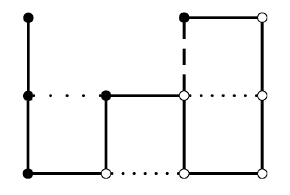
\includegraphics[scale=0.7]{figures/protein_example.png}
	\caption{One possible configuration of  sequence $HHHPHPPPPPH$ in the HP model. There is one $HH$ (represented by a dotted line with wide spaces), one $HP$ (represented by a dashed line) and  two $PP$  (represented by dotted lines) contacts.}
\end{figure}


The total number of topological neighboring positions in the lattice ($z$) is called the lattice coordination number.


For the HP model, an energy function that  measures the interaction between topological  neighbor residues is defined  as  $\epsilon_{HH}=-1$ and $\epsilon_{HP}=\epsilon_{PP}=0$. The HP problem consists of finding the solution that minimizes the total energy. In the linear representation of the sequence, hydrophobic residues are represented with the letter H and polar ones, with P. In the graphical representation, hydrophobic proteins are represented  by black beads and polar proteins, by white beads. Figure~\ref{fig:PROTEXAM} shows the graphical representation of a possible configuration for  sequence  $HHHPHPPPPPH$ in a 2D space. The energy that the HP model associates with this configuration is $-1$ because there is only one $HH$ contact, arisen between the second and fifth residues.


Different heuristic approaches have been developed to decrease the computational complexity related to the protein structure determination process. Mono and Multi-objective methods have been used, trying to define which methods have better results in the study of the PSP Problem.


Among these approaches, there are studies that explore the protein structure prediction combined with evolutionary algorithms like for example, Lin and Su \cite{li2012genetic} proposed an mono objective EA (Evolutionary Algorithm) working with a local search strategy for the PSP Problem using the simplified model Hydrophobic-Polar 2D (HP-2D).


In other work, Lin and Su \cite{lin2011protein} applied a hybrid genetic-based PSO algorithm to HP-3D model with relative representation, optimizing the crossover and mutation operators to improve results in the Protein Folding process. The algorithm was a improved version of a GA based on a PSO, where the solutions were encouraged to move toward their own best solution.


Cust\'{o}dio and Dardenne \cite{custodio2014multiple} proposed a Multiple Minima Genetic Algorithm for PSP. The algorithm included a phenotype based crowding mechanism for the maintenance of useful diversity which increase the population's performance and granted the algorithm multiple solutions capabilities.


Brasil \textit{et al}.\cite{soares2011investigating} proposed an multi objective algorithm in tables and compare its performance with the NSGAII \cite{deb2002fast}, optimizing two energy functions, both very important for the the folding process: the van der Walls and Electrostatic functions.


The author of \cite{gabriel2012algoritmos} also proposes the using of a multi objective algorithm in tables, similar to the proposed method by \cite{soares2011investigating}, however, using the HP model for the representation and solution evaluation.

%----
%TODO ref 19 Roberto
%GA
Unger and Moult \cite{} described a genetic algorithm (GA) that use heuristic-based operators for crossover and mutation for the HP model. The algorithm outperformed many variants of Monte Carlo methods for different instances. Although the good results, the GA was unable to find the optimal solution for the longest instances considered.

%TODO ref 17 Roberto
%MMA
The multimeme algorithm (MMA) proposed by \cite{} is a GA combined with a set fo local searches. The algorithm for each different instance or individuals in the population, select the local search method that best fits. Originally used to find solutions for the functional model protein. The algorithm was later improved with fuzy-logic-based local searches, leading the algorithm to find improved results in the PSP problem.

%TODO ref 25 Roberto
%PERM
Chain growth algorithm as the pruned-enriched Rosenbluth method (PERM) \cite{} is based on growing the sequence conformation by adding individuals particles aiming increase good configurations and eliminating bad ones.

%TODO ref 18 e 28 Roberto
%ACO
The ant colony optimization (ACO) \cite{} is an algorithm that incorporates the use of a modeling step. In this approach, the artificial ants build conformations for a given HP protein sequence, apply a local search to improve the results and maintain a probability value based on the quality of the found solutions, the so called pheromone trail.

\section{Multi-objective Optimization} \label{sec:optimization}


Evolutionary Algorithm (EA) is a optimization and search technique, highly parallel, inspired by the Darwinian principle of natural selection and genetic reproduction. The nature principles that inspire the EAs are simple. According to the theory of C, Darwin, the principle of natural selection favors individuals with high fitness, therefore, with high probability of reproduction. Individuals with more descendants have more chance to perpetuate their genetic code in future generations. The genetic codes is what gives the identity of each individual and are represented in the chromosomes. These principles are used in the construction of computational algorithms, that searches for better solutions given a specific problem by the evolution of a population of solutions coded in artificial chromosomes -- data structures used to represent a feasible solution for a given problem in the algorithm execution \cite{pacheco1999algoritmos}.


Real world problems commonly have multiple objectives to minimize/maximize and are present in most knowledge areas. To optimize multi objective problems, two or more objectives are considered which usually are conflicting. For these problems it is impossible to find one unique solution. A set of solutions is reached evaluating the Pareto dominance relation \cite{pareto} between the solutions. The main goal is to find the solutions that are non-dominated by any other. A solution dominates other, if and only if, it was better in at least one of the objectives, without being worst in any of the objectives. The set of non-dominated solutions constitutes the Pareto Front. Finding the the real Pareto Front is a NP-hard problem \cite{fonseca2005tutorial}, this way, the objective is to find a good approximation of this front.


Multi-Objective Evolutionary Algorithms (MOEAS) are extensions of EAs to multi objective problems that apply the concepts of Pareto dominance to create different strategies to evolve and diversify the solutions. In this work two MOEAs were used: NSGAII \cite{deb2002fast} and IBEA \cite{zitzler2004indicator}.


\subsection{Non-dominated sorting Genetic Algorithm II}


The main characteristic of this algorithm is a strong elitism mechanism, classifying at each generation every solution in different fronts according with the non-dominance relation (line 15 of Algorithm \ref{alg:nsgaII}). After the classification, solutions from the first front, are non-dominated by any other solution. Solutions from the second front are dominated only by the solutions of the first front, and so on. For solutions of the same front, the algorithm uses a Crowding Distance operator to calculate how distant are the neighbors of a given solution (line 19 of Algorithm \ref{alg:nsgaII}). Solutions with high values of Crowding Distance have priority, because they will contribute more to the population's diversity. The binary tournament selects solutions from the small front with the higher values of Crowding Distance. A new population is generated using the crossover and mutation operators (line 25 of Algorithm \ref{alg:nsgaII}).


\begin{algorithm}[htb!]
	\begin{algorithmic}[1]
		\State{$N \gets$ Population Size}
		\State{$T \gets$ Max evaluations}
		\State{$P_0 \gets CreatePopulation(N);$}
		\State{$CalculateFitness(P_0);$}
		\State{$FastNonDominatedSort(P_0);$}
		\State{$Q_0 \gets 0$}
		\While{$Q_0 < N$}
			\State{$Parents \gets BinaryTournament(P_0);$}
			\State{$Children \gets CrossoverMutation(Parents);$}
			\State{$Q_0 \gets Children$}
		\EndWhile
		\State{$CalculateFitness(Q_0);$}
		\State{$t \gets 0$}
		\While{$t < T$}
			\State{$R_t \gets P_t \cup Q_t;$}
			\State{$Fronts \gets FastNonDominatedSort(R_t);$}
			\State{$P_{t+1} \gets 0$}
			\State{$i \gets 0$}
			\While{$P_{t+1} + Front_i  < N$}
				\State{$CrowdingDistanceAssignment(Front_i);$}
				\State{$P_{t+1} \gets P_{t+1} \cup Front_i$}
				\State{$i \gets i + 1$}
			\EndWhile
			\State{$CrowdingDistanceSort(Front_i);$}
			\State{$P_{t+1} \gets P_{t+1} \cup Front_i[1:(N -P_{t+1})]$}
			
			\State{$Parents \gets BinaryTournament(P_{t+1});$}
			\State{$Q_{t+1} \gets CrossoverMutation(Parents);$}
			\State{$t \gets t +1$}
		\EndWhile
		\State{\Return{$P \gets$ Set of non-dominated solutions.}}
	\end{algorithmic}
	\caption{NSGAII}
	\label{alg:nsgaII}
\end{algorithm}


\subsection{IBEA (Indicator-Based Evolutionary Algorithm)}


In the multi-objective optimization context, optimizing consists in find a front with a good approximation to the true Pareto front. However, there is no general definition about what is the true Pareto front. This way, indicators have been used to evaluate the quality of a approximation front. The \textit{hypervolume} is a example of indicator to the evaluation and comparison of fronts.


The IBEA is an algorithm that considers the optimization by the use of quality indicators. The indicator is the way used to evaluate the non-dominated set of solutions \cite{figueiredo2013algoritmo}. To use the IBEA it is necessary define which indicator will be used to associate each ordered pair of solutions to a scalar value. One of the most used indicators is the \textit{hypervolume} due to its capacity of evaluate the convergence and diversity at the same time of the search process \cite{ishibuchi2008evolutionary}.


\begin{equation} \label{eq:ibea_fitness}
	F(x_i) = \sum_{x_j \in (P-x_i)} {-e^\frac{-I_{Hy}(x_j,x_i)}{k}}
\end{equation}


For the IBEA fitness calculation (Equation \ref{eq:ibea_fitness}), $k$ is a parameter commonly used with a value of 0.05. The value for $F(x_i)$ corresponds to a quality loss measure of the approximation to the Pareto front if the solution $x_i$ was removed of the population \cite{figueiredo2013algoritmo}, based on the value of the quality indicator $I_{Hy}$, in this case, the \textit{hypervolume}. Based on the fitness calculation described above, the basic IBEA algorithm consists in iteratively do the selection (line 10 of Algorithm \ref{alg:ibea}), crossover, mutation (line 11 of Algorithm \ref{alg:ibea}) and environment selection, removing the worst individual from the population and updating the values of fitness of the remaining individuals (lines 4 to 8 of Algorithm \ref{alg:ibea}).


\begin{algorithm}[htb!]
	\begin{algorithmic}[1]
	\State{$N \gets$ Population Size}
	\State{$T \gets$ Max Evaluations}
	\State{$k \gets$ Scale factor of Fitness}
	
	\State{$P \gets$ CreatePopulation($N$);}
	\State{$m \gets 0$}
	\State{CalculateFitness($P$);}
	
	\While{$m \ge T$ or other stop criterion is reached}
		
		\State{$\overline P \gets$ BinaryTournament($P$);}
		\State{$P \gets$ CrossoverMutation($\overline P$);}
		\State{$m \gets m+1$}
		
		\While{Size($P$) $> N$}
			\State{$x^* \gets$ WorstIndividualByFitness();}
			\State{RemoveFromPopulation($x^*$, $P$);}
			\State{CalculateFitness($P$);}
		\EndWhile
	
	\EndWhile
		\State{\Return{$P \gets$ Set of non-dominated solutions}}
	
	\end{algorithmic}
	\caption{IBEA}
	\label{alg:ibea}
\end{algorithm}


\footnotetext[1]{\textit{Hypervolume}: Proposed quality indicators used in the study of \cite{zitzler1998multiobjective}, denoted as the "size of the covered search space". This indicator has two important advantages in relation to others \cite{zitzler2007hypervolume}: 1 - Sensitive to any kind of improvement in the approximation set in relation to other set. 2 - As result of 1, the indicator guarantee that for any approximation set $A$ that has high values of hypervolume, also has all the solutions of the true Pareto front.}


\section{Proposed method}
\label{sec:proposedMethod}


Two multi-objective approaches were designed in this chapter, using the MOEAs (NSGAII and IBEA) described on subsection \ref{sec:optimization}. The relative representation was chosen to represent the chromosomes. Integer vectors are used whereas the genes specifies which direction, relative to the previous residue, should be placed the next residue. The genes can assume only tree values (0,1,2), 0 indicates that next residue should be placed on right of the previous one, 1 indicates that the next residue should be placed on left from the previous and 2 indicates that the next residue should be placed in front of the previous one. Figure \ref{fig_sim} shows an example of a hypothetical chromosome and the path generated by it in the 2D lattice.

\begin{figure}[ht]
	\centering
	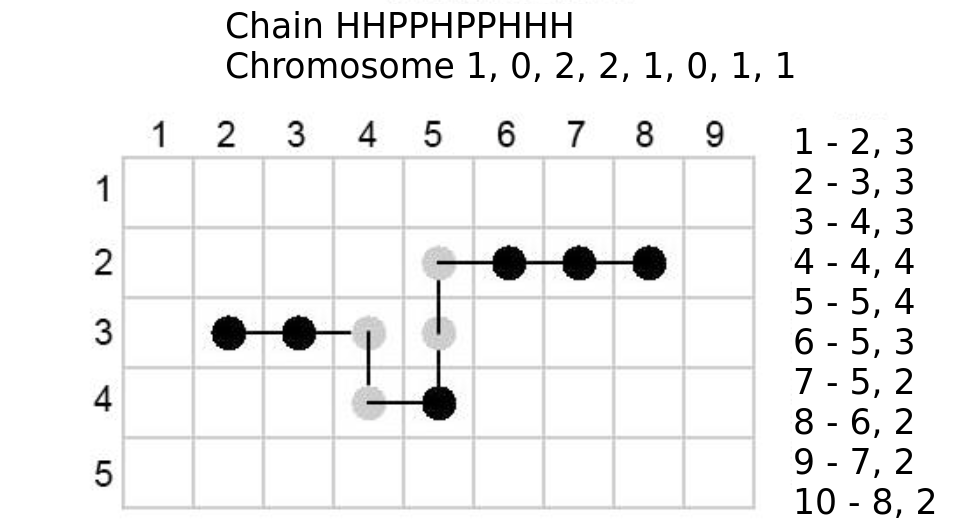
\includegraphics[width=2.5in]{figures/figure3.png}
	\caption{Example of a conformation generated by a chromosome with relative representation.}
	\label{fig_sim}
\end{figure}


The first approach consisted on applying two well-known state of art MOEAs (IBEA and NSGAII) to the PSP using the HP-2D model. The genetic operators used by IBEA and NSGAII algorithms, in this approach, were only the single point crossover in the case of crossover and bit flip mutation for mutation operator.  It was decided to use only single point crossover and bit flip mutation because this combination of operators presented better results in previous experiments realized within the PSP problem and the HP-2D model.

In the case of the second approach the IBEA and NSGAII algorithms were modified in order to improve their results when compared with the first approach. The modifications implemented will be described next:

\begin{itemize}
	\item \textbf{Pool of operators}:  As mentioned in section X, the use of traditional operators usually does not guide the search to prominent regions of the search space of the HP-2D model. In order to supplement the MOEAs, a pool of operators were designed based on the literature and are presented on table X.  For every mating the crossover and mutation operators are selected randomly from the pool of operators and than applied. Also the crossover and mutation operators are always applied differently from the first approach which uses a probability of occurrence. The pool of operators will be described next:
	
	\begin{itemize}
		\item Single Point Crossover (1x): A single point on both parent individuals is selected. All data beyond that point in either individual will be swapped between the two parent individuals. Resulting in two distinct child individuals \cite{holland1975adaptation}.
		
		\item Two Points Crossover (2x): Two points are selected on both parent individuals. Everything between the two points is swapped between the parents. Building two new distinct individuals \cite{holland1975adaptation}.
		
		\item Multi Points Crossover (MPX): The MPX operator is similar to 2X, but the number of points, c, is a function of the sequence length, n, given by $c = int(n \times 0.1)$ \cite{custodio2004investigation}. The MPX operator is usually used to promote structural diversity by performing a random shuffle between individuals, although not as uniform crossover.
		
		\item Bit Flip Mutation (BFM): The BFM operator selects one random gene from a parent individual and changes it to other value. Resulting in one new individual \cite{holland1975adaptation}.
		
		\item Loop Move Mutation (LMM): The LMM operator swaps the directions between two randomly chosen consecutive genes. This operator introduces a corner movement \cite{bazzoli2004memetic}. Figure \ref{fig:operatorLMM} presents a example of application of this operator.
		
		
		
		\begin{figure}[htb!]
			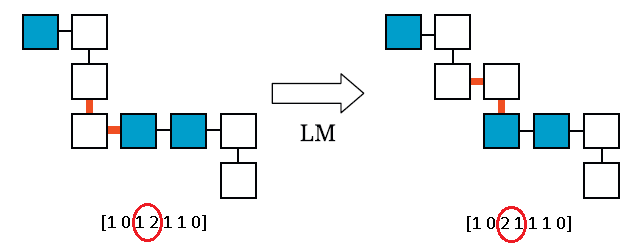
\includegraphics[scale=.6]{figures/operators/LMM.png}
			\label{fig:operatorLMM}
			\caption{Example of application of the LMM operator. The genes from the red circle of leftmost figure were swapped resulting in the rightmost figure.} 
		\end{figure}
		
		\item Loop Move Mutation (LoMM): This operator is similar with LMM however exchanges directions between genes that are five positions apart on the sequence creating a loop movement. Both LMM and LoMM is useful to generate modifications on compact structures \cite{custodio2014multiple}.
		
		%Adicionar figura LoMM
		
		\item Segment Mutation (SM): This operator changes a random number of consecutive genes (from two to seven) into new random directions. This operator introduces large conformational changes and has a high probability of creating collisions, in order to avoid too much invalid solutions the repair mechanism is applied on the generated child \cite{custodio2014multiple}. 
		
		%Adicionar FIGURA SM
		
		\item Opposite Mutation (OM): This operator changes a random number of consecutive genes to its inverse position. In the case of the relative representation to the HP-2D model, only left and right can be mapped to its inverse.  
		
		%Adicionar FIGURA OPPOSITE
		
		
		
	\end{itemize}

	
	\item \textbf{Backtrack Initialization}: Traditionally the initial population of solutions are generated randomly in the presented MOEAs. This have a great potential of generating a large number of invalid solutions for the PSP problem within the HP-2D model. Solutions that are not self-avoiding walk (SAW) are said to contain collisions. If the initial population is fully generated randomly the evolutionary algorithms will spend time processing invalid solutions until getting good results. In order to subdue this problem a backtrack strategy should be applied. In this approach 20 percent of the initial population were generated using the backtrack initialization.
	
\end{itemize}

For both approaches the same objectives were used and will be explained  at next:

\begin{itemize}
	\item \textbf{Energy value}: This is the main objective and consist in the energy of given protein conformation.  The goal is to minimize the energy value and it is calculated as described in section X. This objective guides the search progress towards regions that the energy associate to the protein conformations are minimal. Thus, achieving protein conformations which are closest to native structure of a protein.
	\item \textbf{Distance between the two farthest residues}: This is a secondary objective and it was inspired by the related work X. The motivation for this objective is that more compact conformations tend to have more hydrophobic contacts which means a lesser energy value. The distance between two residues is calculated using the Euclidean distance.
\end{itemize}




The relative representation it is subject to generation of invalid solutions using the HP-2D model. A solution is considered invalid when the solution does not perform a self-avoiding walk (SAW) as mentioned before. In other words a invalid solution is when a given residue collides with another already placed on the lattice. A simple mechanism for repairing these situations was developed, the code can be seen in the Algorithm \ref{algo:reparacao}.

\begin{algorithm}[h]
	1. Obtains the direction that next residue should be placed.\\
	2. Verifies if this direction will cause collision.\\
	3. If the a collision is detected, a new direction is used.\\
	4. Repeat the step 2 and 3, until be possible to place the next residue, or if all directions were tested and cause collisions.\\
	5. If was possible to place the next residue, the mechanism achieved success, if not, the solution is considered infeasible and it will be penalized in the evaluation process.
	\caption{Mechanism to repair infeasible solutions}
	\label{algo:reparacao}
\end{algorithm}

This mechanism was implemented because in previous experiments was observed that the number of infeasible solutions was too big. It is necessary mention that the even with the mechanism to repair solutions, there are still infeasible solutions because the mechanism can not always repair. Thus, infeasible solutions are penalized by subtracting the number of collisions to the quantity of topological neighbors. This mechanism is used by the evaluation process of both approaches described before (IBEA and NSGAII without any major modifications and the same algorithms with the modifications mentioned).

To evaluate and compare the performance of multi-objective algorithms, quality indicators are commonly used. In this study was used the hypervolume indicator, which considers the volume of the search space dominated by the known pareto front \cite{zitzler2003performance} of an algorithm. Higher hypervolume value means that the quality is better than one lesser hypervolume value.

\section{Experiments}

This section presents the set of experiments designed to evaluate the performance of the approaches introduced in section \ref{sec:proposedMethod}. The HP sequences used in the experiments are shown in table \ref{tab:instances}, those instances have been used in previously works such as \cite{bastolla1997testing,shmygelska2002ant,unger1993genetic,cotta2003protein, santana2004protein,shmygelska2003improved,lesh2003complete}. The values presented in table \ref{tab:instances} correspond to the sequence identifier, the size of aminoacid sequence, the best known solutions ($H(x*)$) for the HP-2D model and the sequence itself. 

\begin{table}[htbp]
	\begin{center}
		\caption{HP instances used in the experiments. The search space of each instance is $2^n$ where $n$ is the size of
			the instance.}
		\label{tab:instances}
		{$\begin{array}{c r r l}
			\text{inst.} & \text{size} &  \multicolumn{1}{ c }{H({\bf{x}}^*)} & \multicolumn{1}{c}{\text{sequence}} \\ \hline
			s1 &20 &-9 & HPHPPHHPHHPHPHHPPHPH \\
			s2 &24 &-9 & HHPPHPPHPPHPPHPPHPPHPPHH \\
			s3 &25 &-8 & PPHPPHHP^4HHP^4HHP^4HH \\
			s4 &36 &-14 &  P^3HHPPHHP^5H^7PPHHP^4HHPPHPP\\
			s5 &48 &-23 &  PPHPPHHPPHHP^5H^{10}P^6 \\
			&   &    &  HHPPHHPPHPPH^5 \\
			s6 &50 &-21 &  HHPHPHPHPH^4PHP^3HP^3HP^4 \\
			&   &    & HP^3HP^3HPH^4{\{PH\}}^4H\\
			s7 &60 &-36 &  PPH^3PH^8P^3H^{10}PHP^3\\
			&   &    &  H^{12}P^4H^6PHHPHP\\
			s8 &64 &-42 &   H^{12}PHPH{\{PPHH\}}^2PPH{\{PPHH\}}^2\\
			&   &    &  PPH{\{PPHH\}}^2PPHPHPH^{12}\\
			s9  &85   &-53  & H^4P^4H^{12}P^6 H^{12} P^3 H^{12} P^3 \\
			&   &    &    H^{12} P^3  H P^2 H^2    P^2 H^2  P^2 H P H  \\
			s10  &100  &-48  &  P^6HPH^{2}P^5H^{3}PH^5PH^{2} P^4 H^{2} \\
			&   &    &   P^2  H^2 P  H^5  P H^{10} P H^{2} P H^{7}  \\
			&   &    &  P^{11} H^{7} P^2  H P   H^3  P^{6} H P H \\
			s11 &100  &-50  &  P^3H^{2}P^2H^{4}P^2H^{3}PH^{2} PH^{2}PH^{4} \\
			&   &    & P^8 H^6 P^{2} H^{6} P^{9} H P H^{2} P  H^{11} P^2  \\
			&   &    &H^3 P  H^{2} P H P^2  H P H^3 P^6 H^3\\ \hline
			\end{array}$}
	\end{center}
\end{table}

\subsection{Results for both approaches and the results from previous works}



\section{Conclusion}